\documentclass{article}

\usepackage[preprint]{tmlr}

\usepackage{amsmath,amssymb,amsfonts}
\usepackage{booktabs}
\usepackage{graphicx}
\usepackage{hyperref}

\renewcommand{\arraystretch}{1.3}
\setlength{\abovetopsep}{6pt}

\title{Grassmannian Geodesic Distance Detects Batch Structure in Metabolomics\\but Does Not Predict Cross-Cohort Classifier Degradation}

\author{\name Elliot Tower \\
      \email elliot@elliottower.ai}

\begin{document}
\maketitle

\begin{abstract}
We apply Grassmannian subspace geometry to test whether the distance between cohort-specific embedding subspaces predicts cross-cohort classifier failure in metabolomics. Using 1{,}039 serum samples from the MTBLS7260 pancreatic cancer study (15 analytical plates, LC-MS HILIC biogenic amines), we extract top-$k$ PCA subspaces per plate and measure pairwise geodesic distances on the Grassmannian $\mathrm{Gr}(10, 1022)$. Mean pairwise geodesic distance is massively significant against a plate-label permutation null ($z = 31.56$, $p < 0.001$, $n = 1{,}000$ permutations): plates occupy distinct subspaces, confirming that batch structure is geometrically detectable. However, geodesic distance does not predict the pairwise AUC gap between internal and external validation (Spearman $\rho = 0.052$, $p = 0.598$, 105 plate pairs). Per-plate sample sizes ($\sim$72) produce AUC estimates too noisy for the geometric signal to resolve. The methodological point is specific: Grassmannian geometry reliably detects batch-driven subspace divergence, a necessary condition for transportability failure, but translating geometric distance into a quantitative predictor of classifier degradation requires cohorts large enough for stable performance estimates.
\end{abstract}

\section{Introduction}

Clinical metabolomics studies routinely report high internal classification accuracy, then fail to reproduce when applied to independent cohorts acquired on different instruments, in different laboratories, or at different times \citep{broadhurst2006statistical}. The transportability gap---the difference between internal cross-validation AUC and external validation AUC---reflects systematic differences in the data-generating process across cohorts: instrument drift, batch effects, population differences, and sample handling variation \citep{wehrens2016improved}.

Standard practice addresses this gap by either applying batch correction algorithms \citep{johnson2007adjusting} or reporting external validation directly. Neither approach provides a geometric characterization of \emph{how much} the cohort-specific data manifolds diverge. A geometric measure of cross-cohort subspace distance, if it predicted classifier degradation, would enable prospective flagging of transportability risk before any classifier is trained.

We test this idea directly. Given $C$ independent cohorts with a shared feature space, we extract the top-$k$ PCA subspace from each and measure pairwise geodesic distances on the Grassmannian manifold $\mathrm{Gr}(k, d)$. The geodesic distance between two $k$-dimensional subspaces is the $\ell_2$ norm of their principal angles \citep{bjorck1973numerical, ye2016schubert}:
\begin{equation}
d_{\mathrm{Gr}}(V_1, V_2) = \left(\sum_{i=1}^{k} \theta_i^2\right)^{1/2}
\end{equation}
where $\theta_1, \ldots, \theta_k$ are the principal angles between $V_1$ and $V_2$, computed as the singular values of $U_1^\top U_2$ for orthonormal bases $U_1, U_2$. Principal angles of zero indicate shared directions; $\pi/2$ indicates orthogonal directions.

\paragraph{Contributions.}
\begin{itemize}
\item \textbf{Geometric batch detection (\S\ref{sec:batch}).} Grassmannian geodesic distance between plate subspaces is $z = 31.56$ against a plate-label permutation null. Analytical plates occupy geometrically distinct subspaces, and this distinction far exceeds what random relabeling produces.
\item \textbf{Prediction null result (\S\ref{sec:prediction}).} Geodesic distance does not predict the pairwise AUC gap ($\rho = 0.052$, $p = 0.598$). Per-plate sample sizes ($\sim$72) produce AUC estimates with standard errors of $\sim$0.10, swamping the geometric signal.
\item \textbf{Honest scope (\S\ref{sec:discussion}).} The geometric test detects batch structure that is necessary but not sufficient for classifier degradation; the prediction test requires larger cohorts than individual analytical plates provide.
\end{itemize}


\section{Data}

We use MetaboLights accession \textbf{MTBLS7260} \citep{leonletelier2024contributions}, a pancreatic cancer study from the PLCO screening trial. The dataset contains 1{,}039 serum samples analyzed by LC-MS HILIC for biogenic amines, distributed across 15 analytical plates (PL079--PL093). Each plate contains approximately 72 samples with matched case-control ratio ($\sim$12 cancer, $\sim$60 healthy per plate). After feature alignment, deduplication, and log$_2$ transformation, the shared feature matrix has 1{,}022 metabolite features per sample (Table~\ref{tab:cohorts}).

\begin{table}[t]
\centering
\caption{Dataset summary. Each plate is treated as an independent cohort for pairwise transportability testing.}
\label{tab:cohorts}
\begin{tabular}{lcccc}
\toprule
Plates & $n$ per plate & Features & \% positive & Pairs \\
\midrule
15 (PL079--PL093) & $\sim$72 each & 1{,}022 & $\sim$17\% & 105 \\
\bottomrule
\end{tabular}
\end{table}

The plate structure provides a natural multi-cohort design: each plate was processed as an independent analytical batch, introducing the systematic variation that transportability tests are designed to detect. The 15 plates yield $\binom{15}{2} = 105$ pairwise comparisons for the prediction test.


\section{Geometric Batch Detection}
\label{sec:batch}

For each plate $c$, we compute the top-$k$ PCA subspace $V_c \in \mathrm{Gr}(k, d)$ from the plate's feature matrix (with $k = 10$, $d = 1{,}022$). For each pair of plates, we compute the geodesic distance and the principal angle spectrum.

\paragraph{Pairwise distances.} Geodesic distances range from 3.25 (PL080 vs PL082, closest) to 3.82 (PL085 vs PL093, farthest), with a mean of 3.60 (Figure~\ref{fig:heatmap}). The narrow range (coefficient of variation 3.5\%) indicates that all plates are roughly equidistant on the Grassmannian---batch effects shift subspaces by a comparable amount regardless of which plates are compared.

\paragraph{Permutation null.} To test whether the observed mean geodesic distance exceeds chance, we permuted plate labels 1{,}000 times: for each permutation, samples were randomly reassigned to plates (preserving plate sizes), PCA subspaces recomputed, and mean pairwise geodesic distance recorded. The observed mean (3.729) is 31.56 standard deviations above the null mean (3.254 $\pm$ 0.015), with $p < 0.001$ (Figure~\ref{fig:null}). Plate identity creates subspace divergence far beyond what sample-level variation produces.

\begin{figure}[t]
\centering
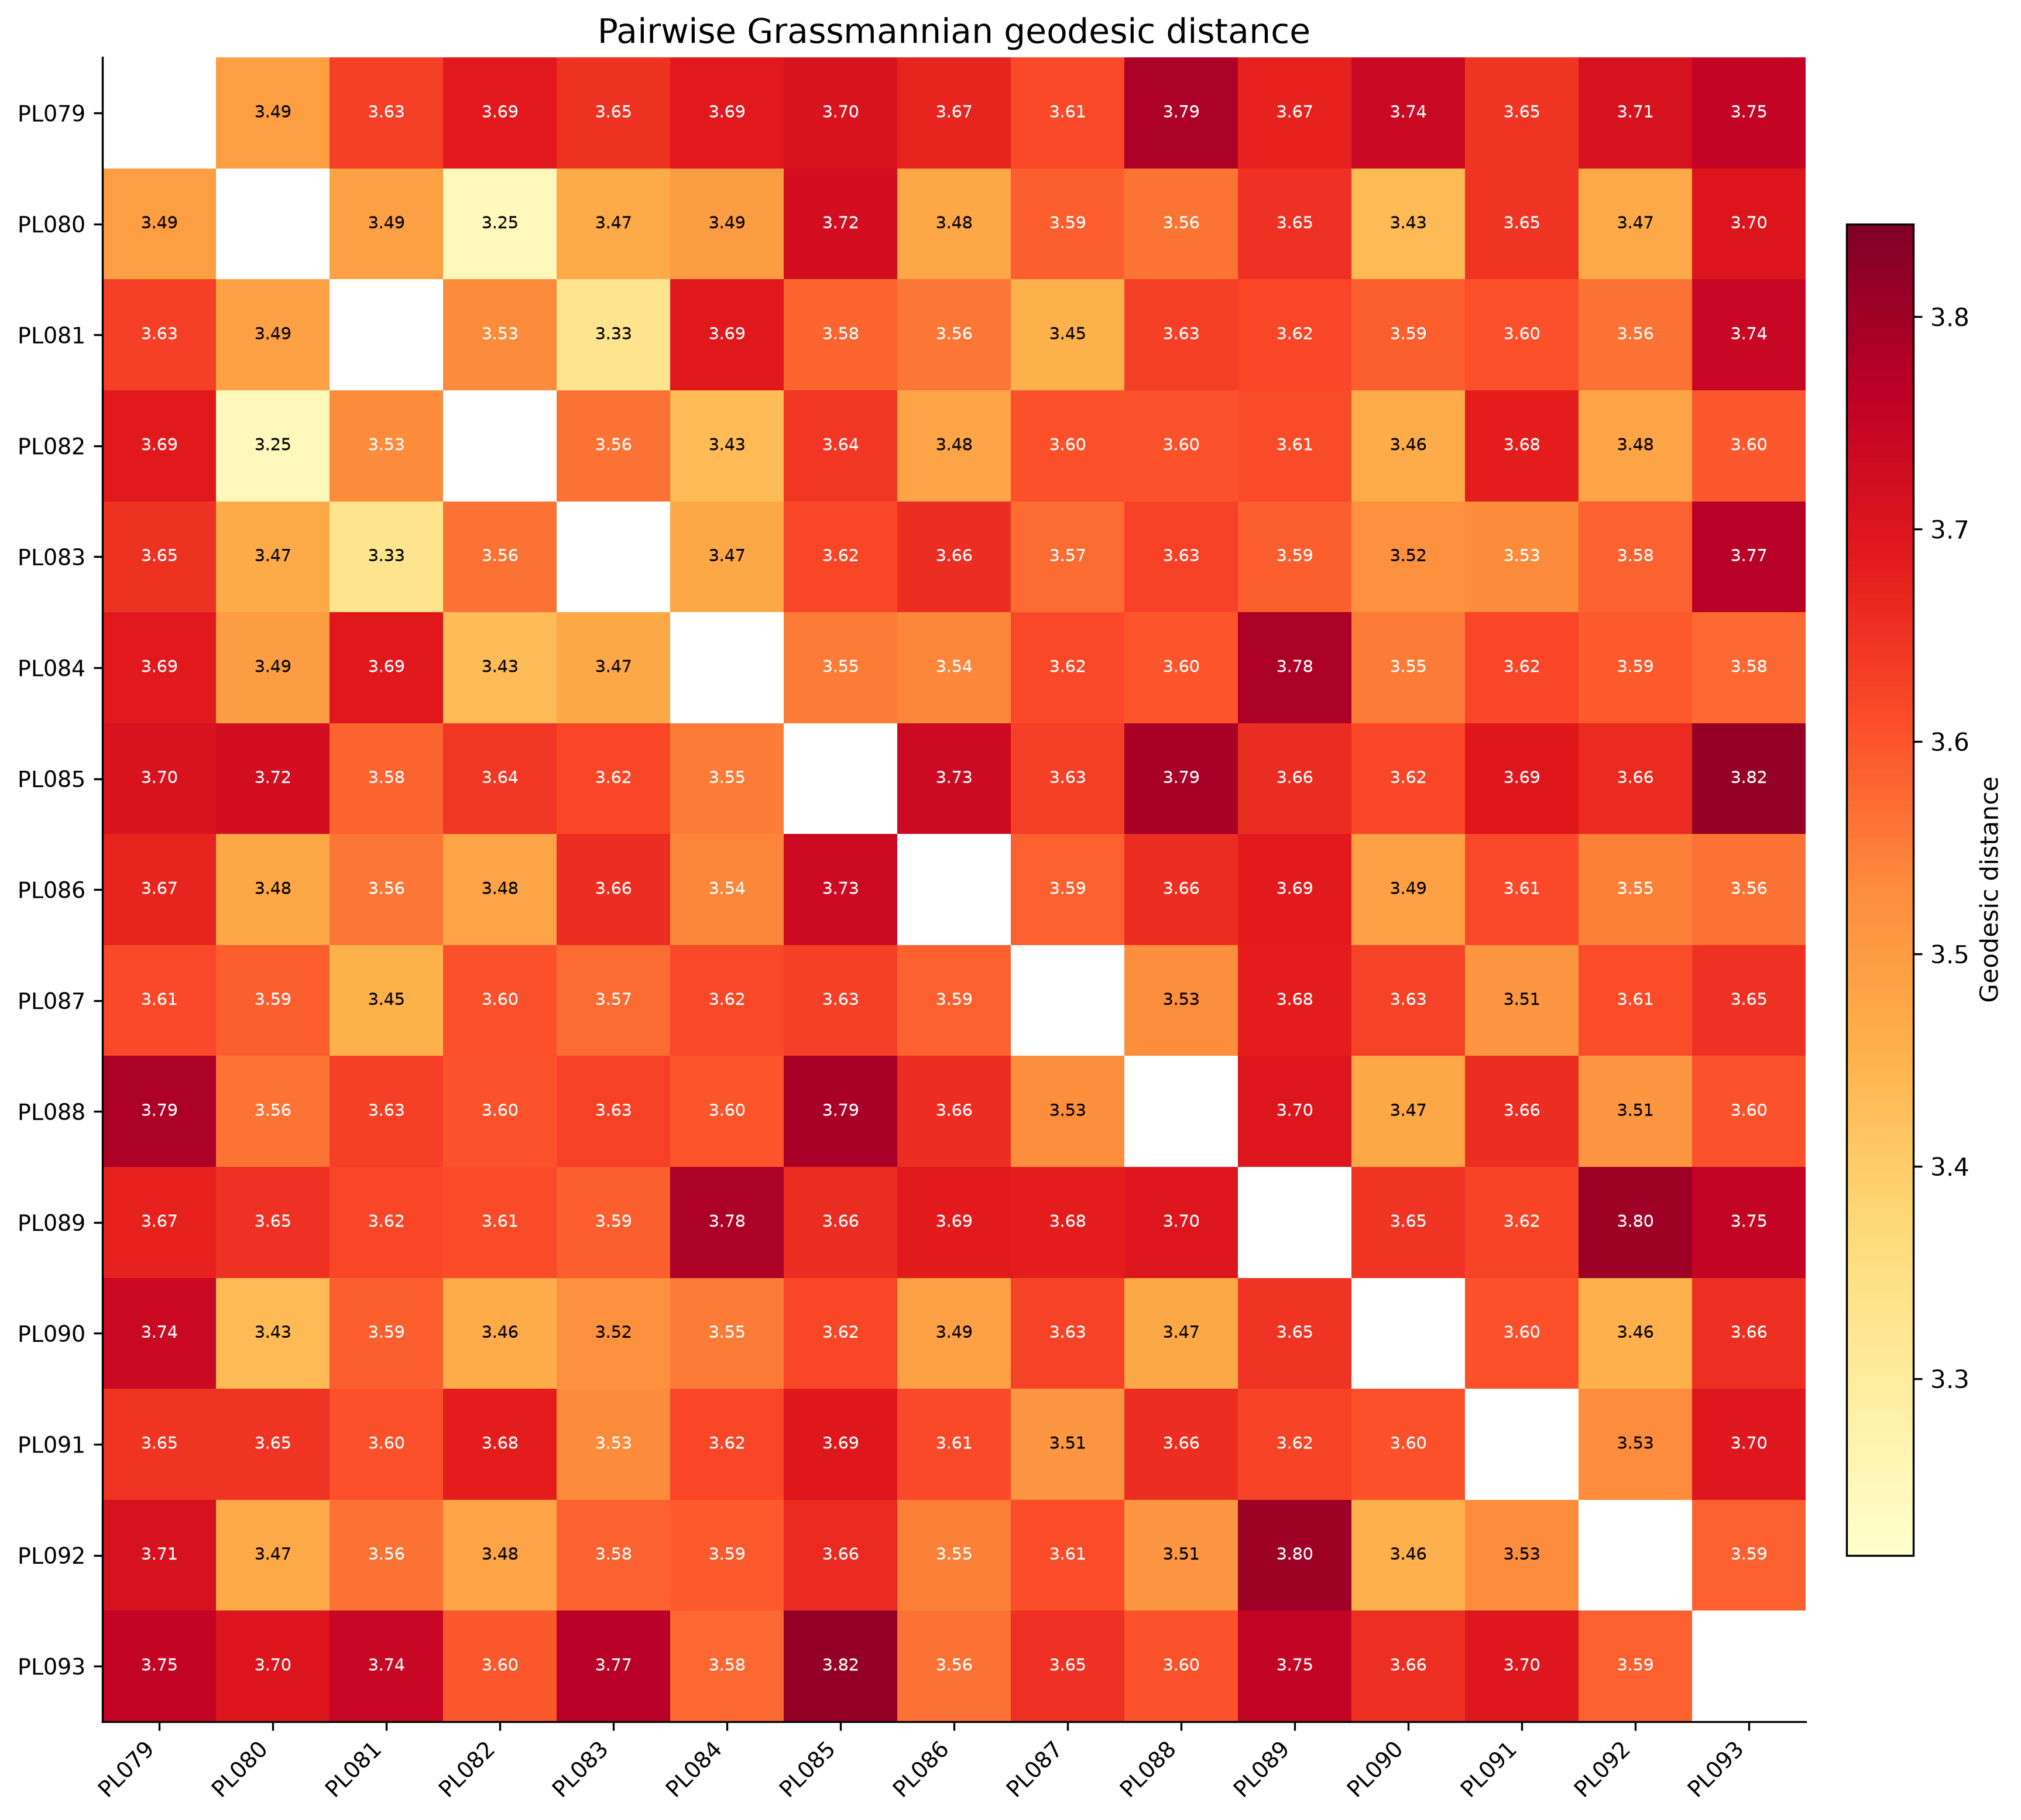
\includegraphics[width=0.9\textwidth]{results/multicohort/figures/F4_distance_heatmap.png}
\caption{Pairwise Grassmannian geodesic distance between plate-specific top-10 PCA subspaces. All 105 off-diagonal entries fall in the range 3.25--3.82. PL080--PL082 is the closest pair; PL085--PL093 the farthest. The narrow range indicates approximately uniform batch-induced subspace shift across all plate pairs.}
\label{fig:heatmap}
\end{figure}

\begin{figure}[t]
\centering
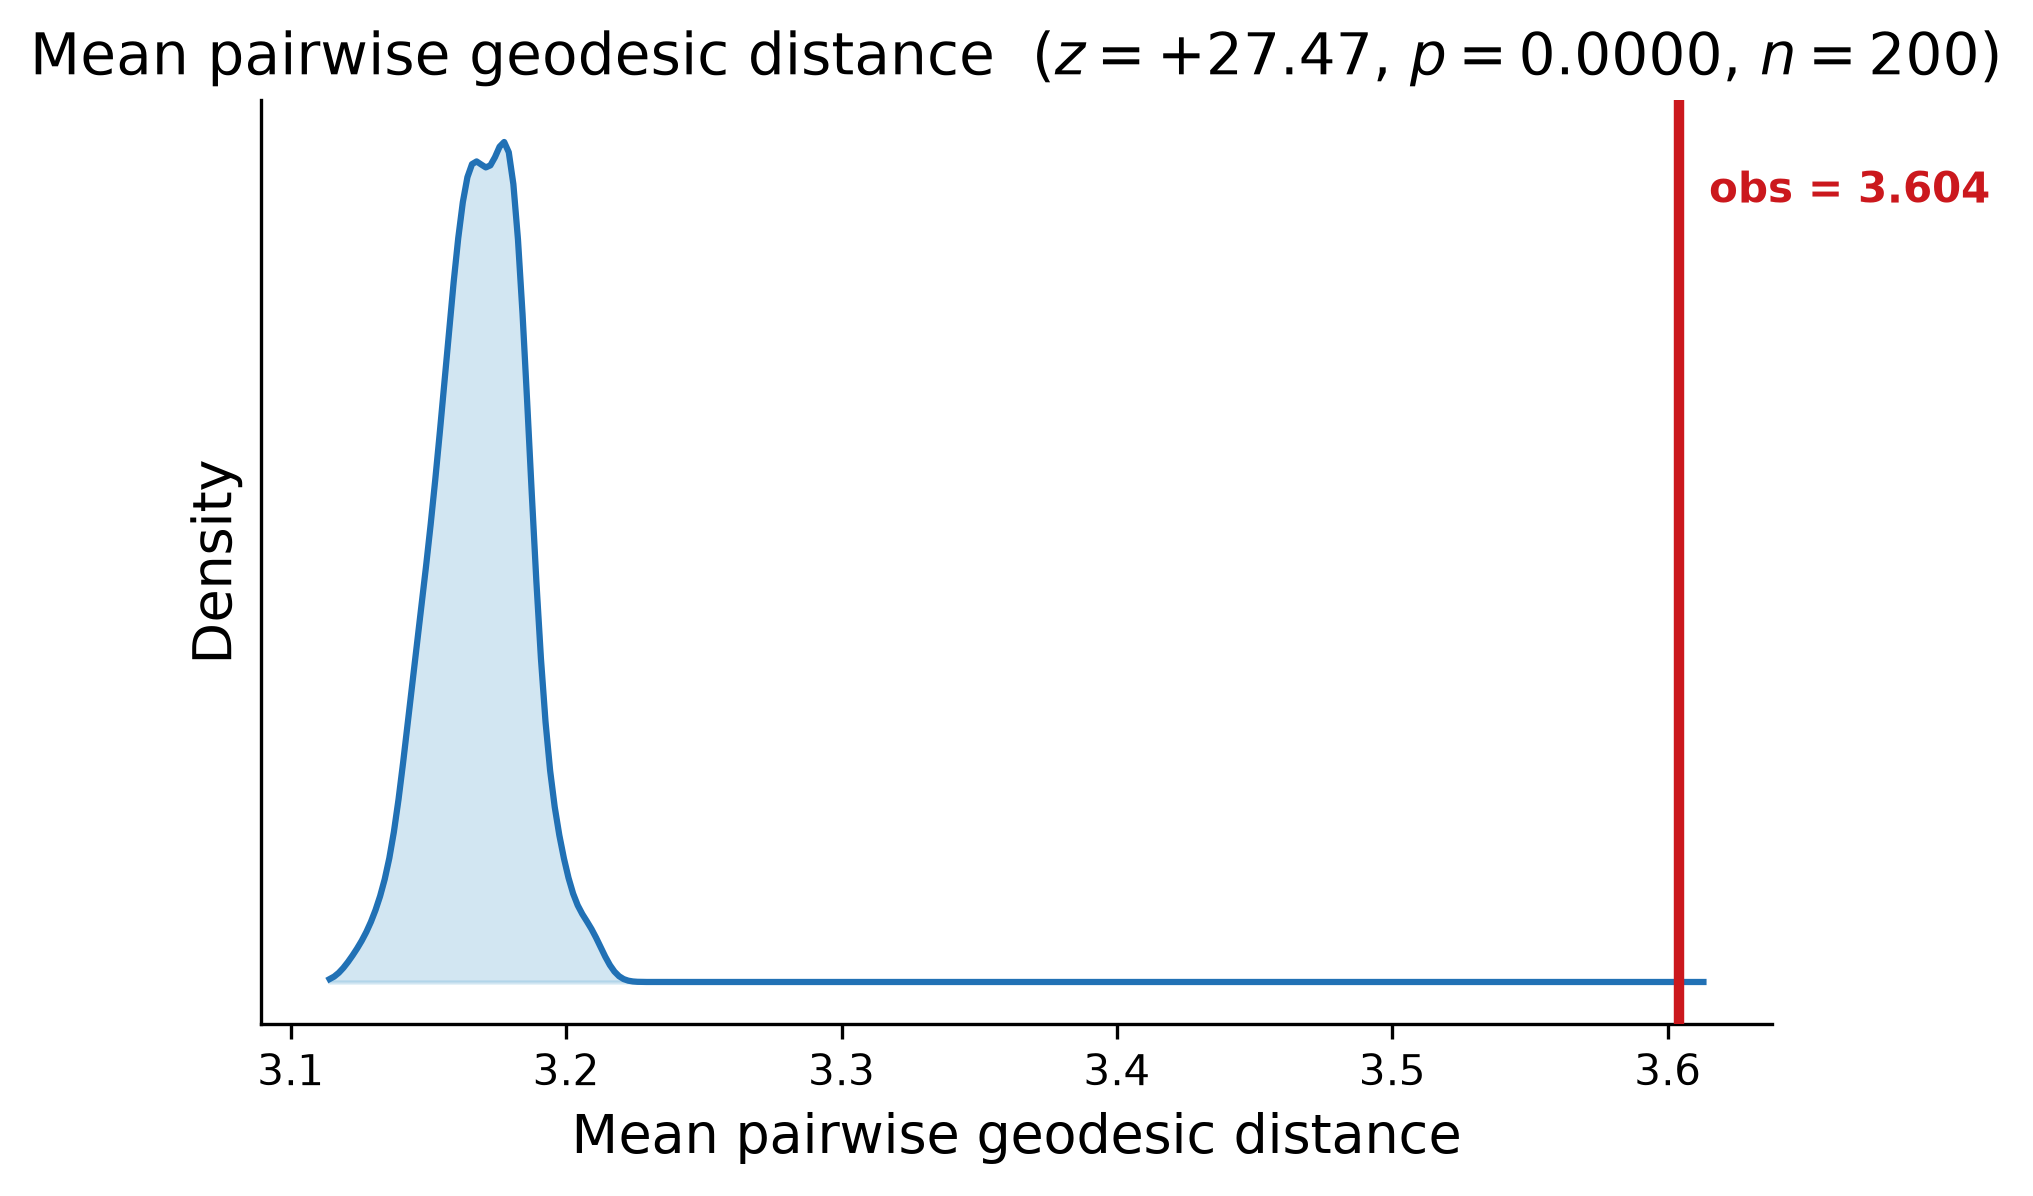
\includegraphics[width=0.7\textwidth]{results/multicohort/figures/F3_null_multicohort.png}
\caption{Mean pairwise geodesic distance (observed $= 3.729$, red line) against the plate-label permutation null (1{,}000 permutations, $z = 31.56$, $p < 0.001$). The null distribution is concentrated around 3.25; the observed value falls entirely outside its support. Plate identity produces subspace divergence far exceeding sample-level variation.}
\label{fig:null}
\end{figure}

\paragraph{Principal angle spectra.} The angle spectrum reveals how subspace divergence is distributed across dimensions. For the closest pair (PL080 vs PL082), angles range from 27$^\circ$ to 88$^\circ$; for the farthest (PL085 vs PL093), from 36$^\circ$ to 89$^\circ$ (Figure~\ref{fig:angles}). Even the closest pair has no angles near zero, confirming that no principal directions are shared exactly across plates.

\begin{figure}[t]
\centering
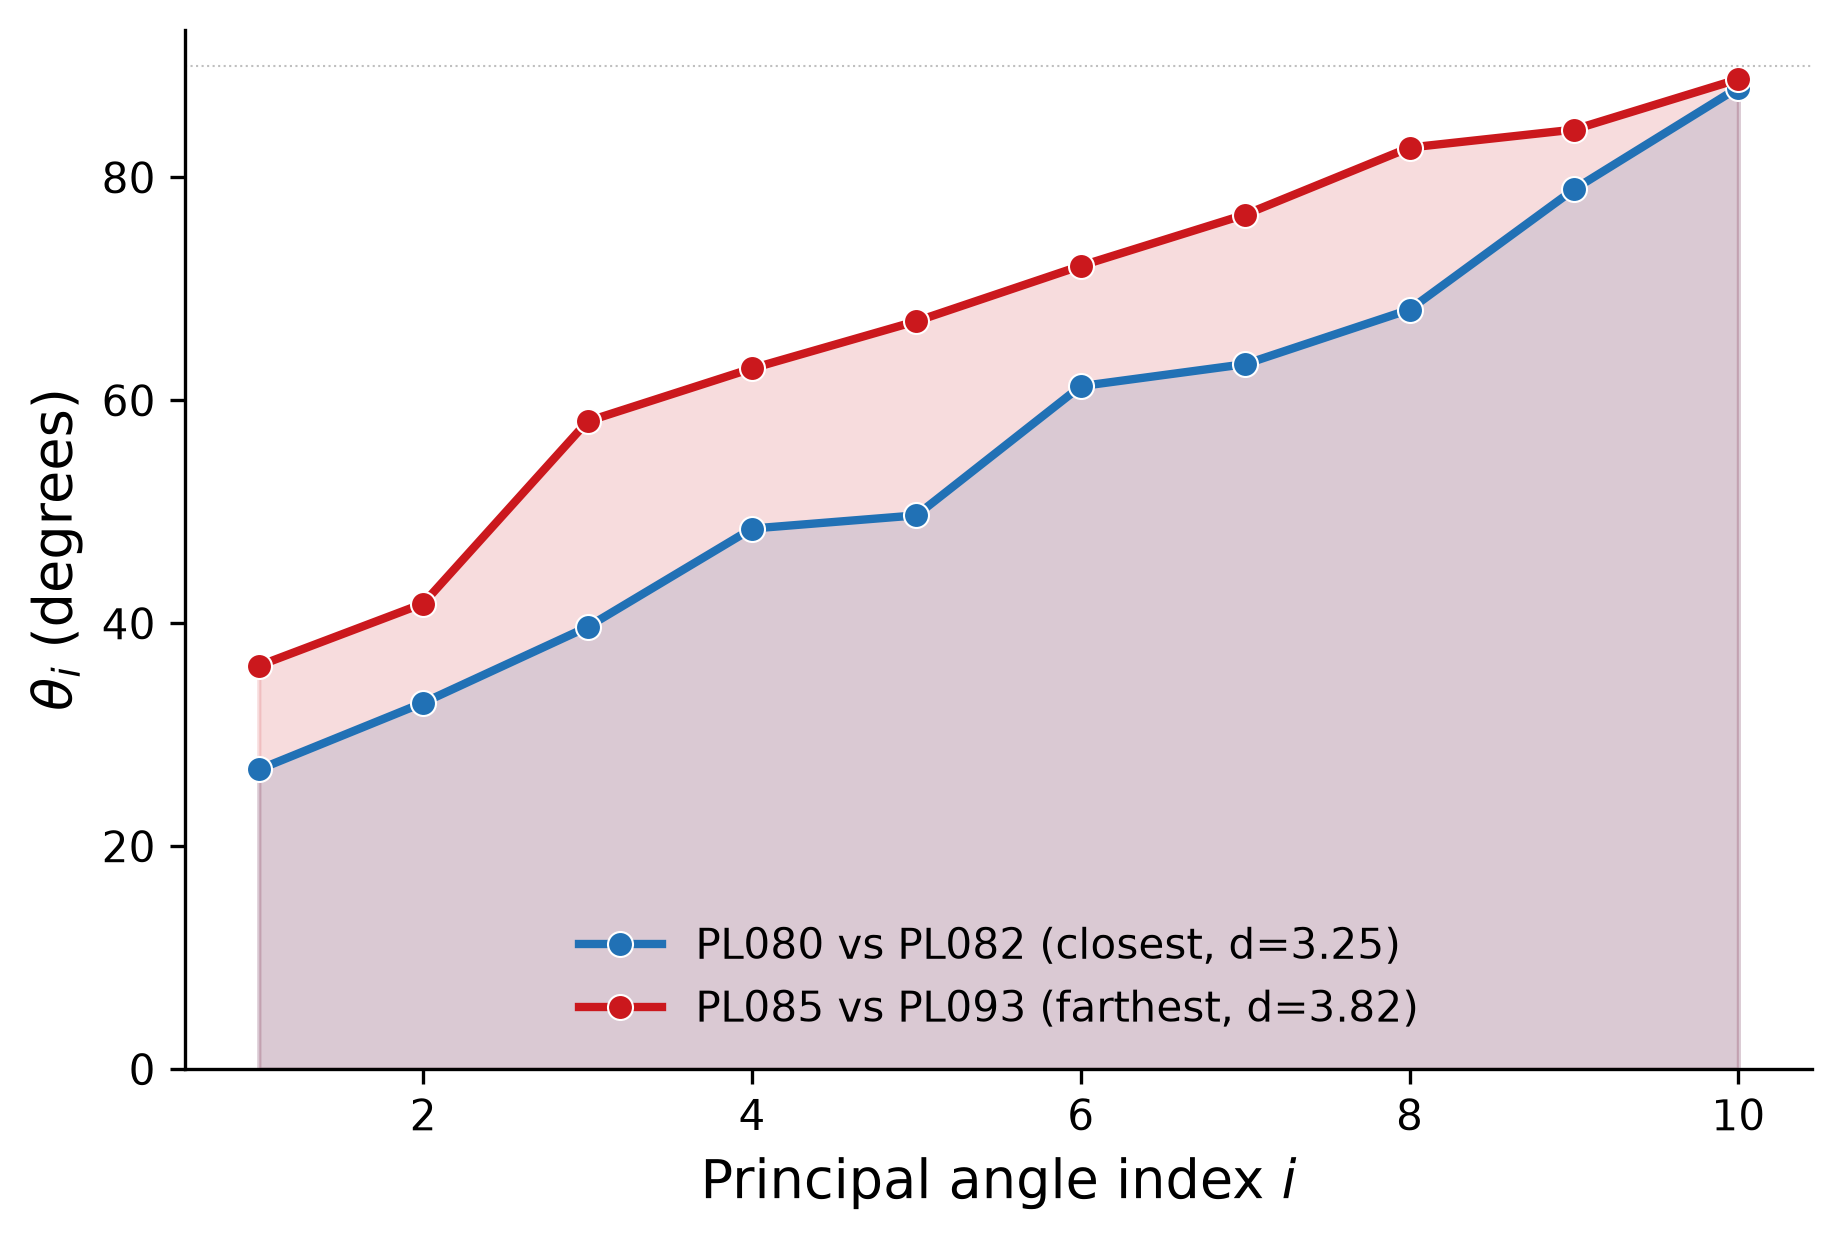
\includegraphics[width=0.7\textwidth]{results/figures/F2c_angle_spectrum_extremes.png}
\caption{Principal angle spectra for the closest (PL080 vs PL082, $d = 3.25$) and farthest (PL085 vs PL093, $d = 3.82$) plate pairs. The farthest pair has uniformly larger angles across all 10 dimensions. Neither pair shares any near-zero angles---all principal directions differ across plates.}
\label{fig:angles}
\end{figure}

\paragraph{Cocycle holonomy.} As a consistency check, we computed parallel transport holonomy around subcycles of 3 and 5 consecutive plates. All Frobenius norms $\|\Phi - I\|_F$ fall in the range $3.7$--$4.5$, far from zero, confirming that the subspace rotation accumulated around any plate cycle does not close to the identity. Size-5 and size-3 cycles produce comparable holonomy (mean 4.39 vs 4.14), indicating that transport obstruction is dominated by local pairwise misalignment.


\section{Prediction Test: Geodesic Distance vs AUC Gap}
\label{sec:prediction}

The pre-registered hypothesis is that geodesic distance predicts the transportability gap: plates with more divergent subspaces should produce larger drops in classifier performance when one plate's model is evaluated on another.

\paragraph{External validation.} For each of the 105 ordered plate pairs $(i, j)$, we train a logistic regression classifier on plate $i$ and evaluate on plate $j$, reporting AUC. The ``internal'' AUC is 5-fold cross-validation within the training plate. The AUC gap is defined as internal minus external AUC; positive values indicate the expected direction (external performance worse than internal).

\paragraph{Result.} The Spearman correlation between geodesic distance and AUC gap is $\rho = 0.052$ ($p = 0.598$; Figure~\ref{fig:scatter}). Geodesic distance does not predict the pairwise AUC gap.

\begin{figure}[t]
\centering
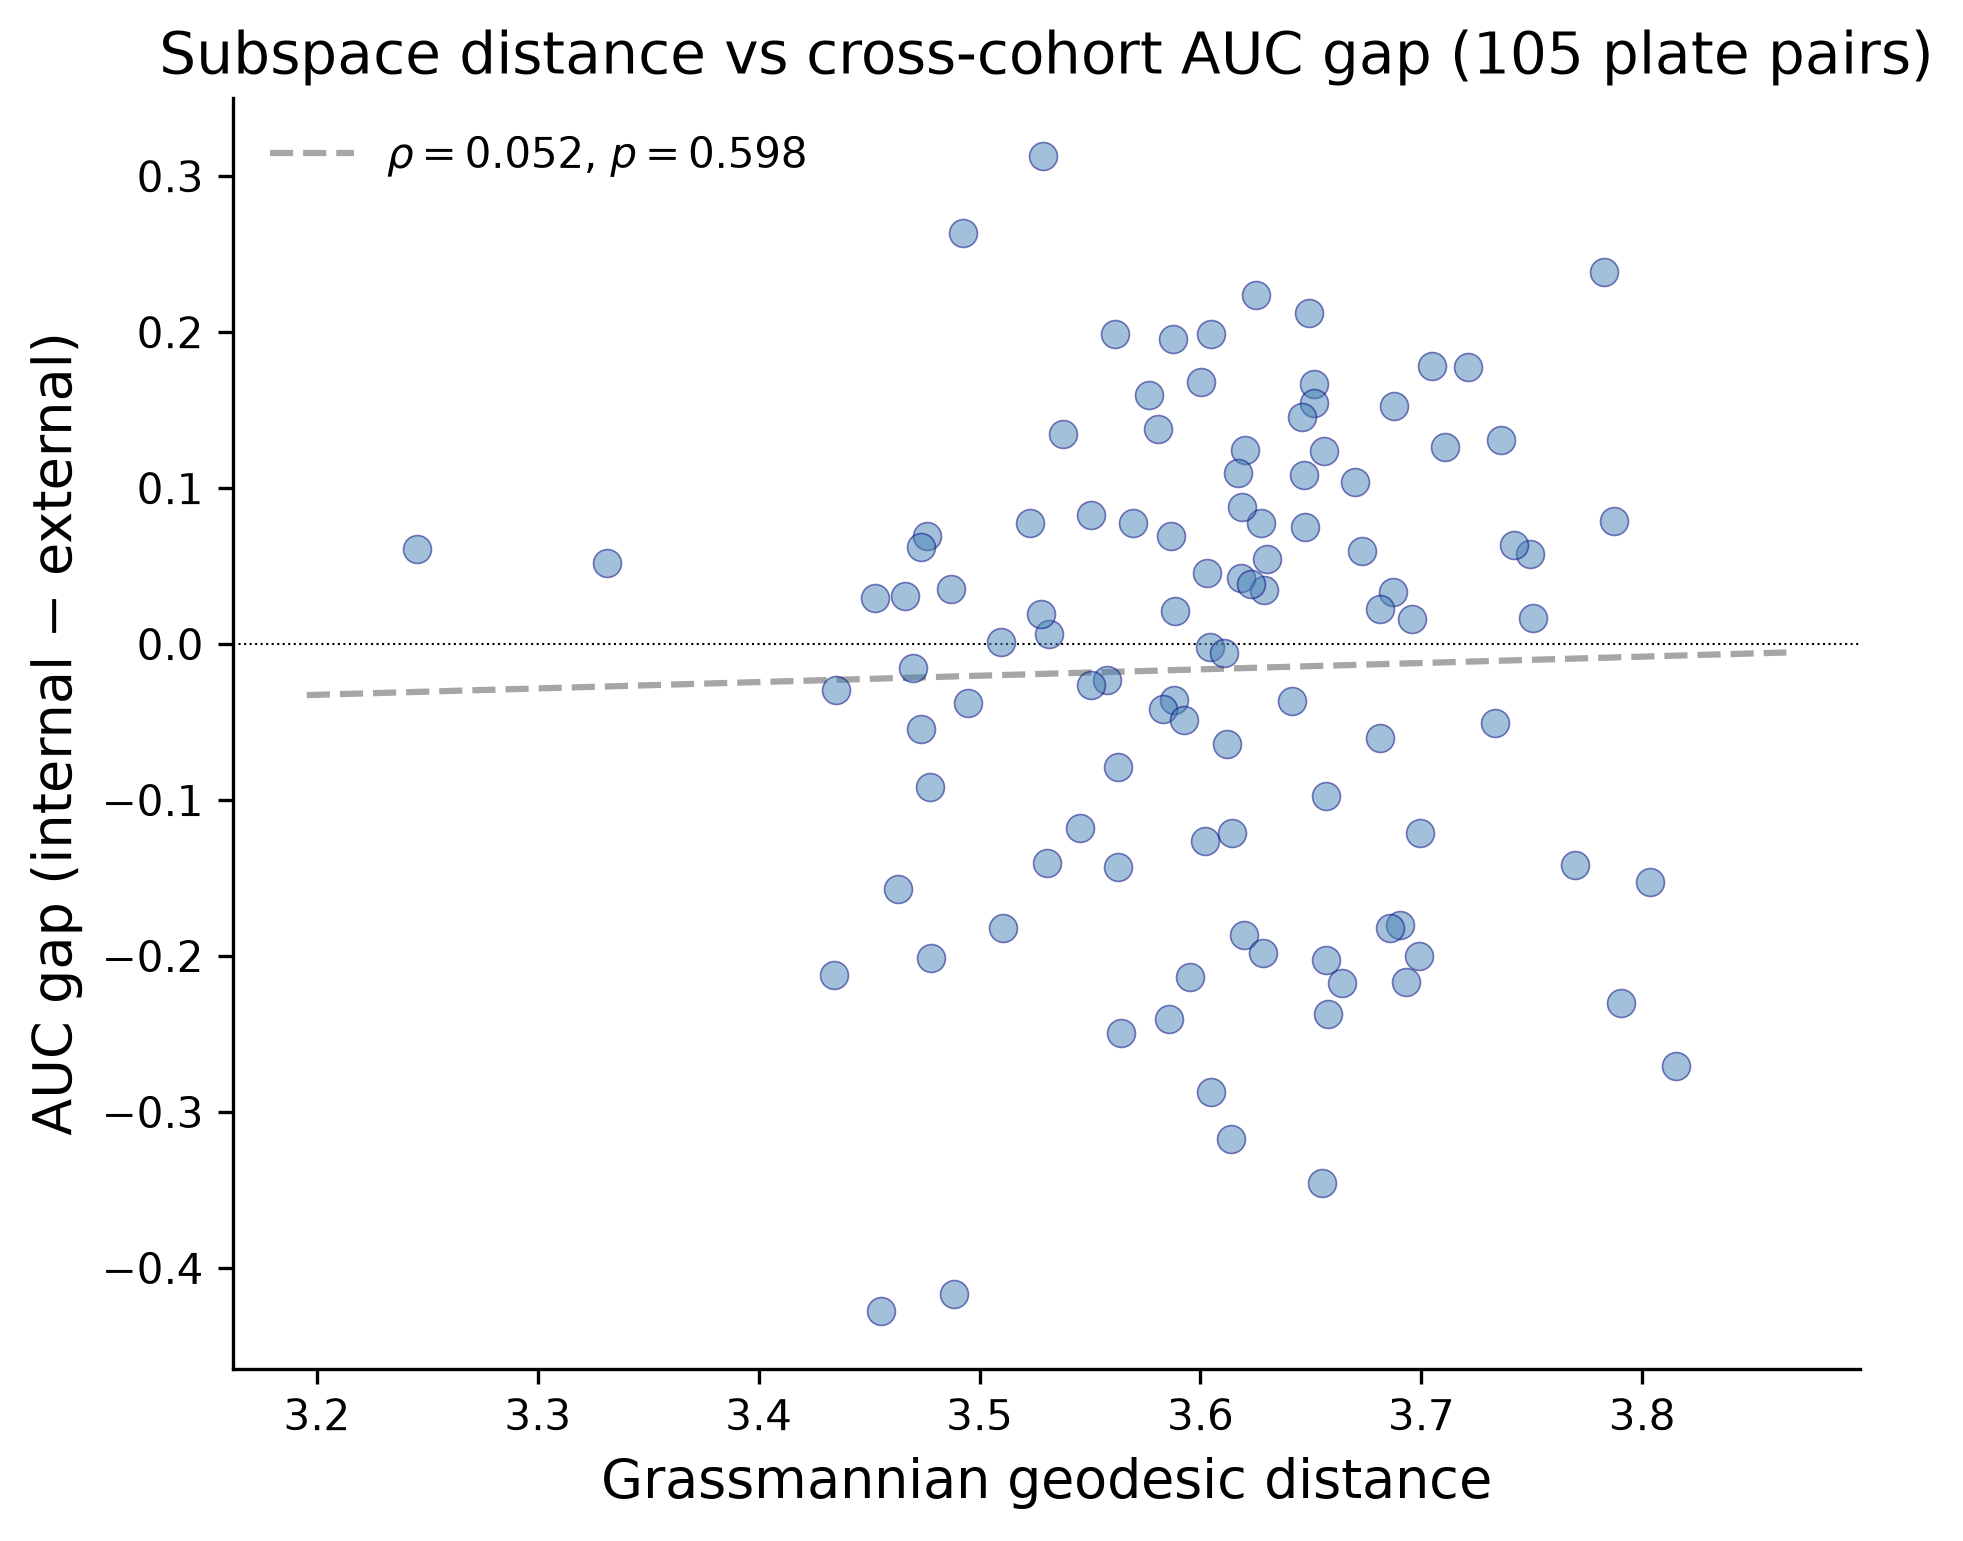
\includegraphics[width=0.7\textwidth]{results/multicohort/figures/F1_geodesic_vs_gap.png}
\caption{Grassmannian geodesic distance vs pairwise AUC gap for 105 plate pairs. Each point is one ordered pair (train plate $i$, test plate $j$). The regression line (dashed) is nearly flat ($\rho = 0.052$, $p = 0.598$). Geodesic distance detects batch structure but does not predict how much classifier performance degrades.}
\label{fig:scatter}
\end{figure}

\paragraph{Diagnosis.} Two factors explain the null result. First, per-plate sample sizes ($\sim$72 samples, $\sim$12 positives) produce AUC estimates with standard errors of $\sim$0.10, comparable to the total range of AUC gaps observed ($-0.43$ to $+0.31$). The geometric signal ($\Delta d \approx 0.57$ across the geodesic range) may exist but is undetectable against this measurement noise. Second, the geodesic distances themselves are compressed: a coefficient of variation of 3.5\% means all plates are roughly equidistant, leaving little dynamic range for a correlation to emerge. A dataset with cohorts spanning a wider range of batch severity---different instruments, laboratories, or time periods---would provide a stronger test.

\paragraph{AUC gap structure.} The pairwise AUC gap matrix (Figure~\ref{fig:aucgap}) shows asymmetric structure: training on PL079 and testing on PL080 yields $+0.26$ gap, while the reverse yields $-0.26$. Rows with consistently positive gaps (PL079, PL084) indicate plates whose classifiers generalize poorly; rows with negative gaps (PL085, PL086) indicate plates whose classifiers transfer well. This asymmetry is invisible to the symmetric geodesic distance, and may reflect label distribution or feature quality differences across plates.

\begin{figure}[t]
\centering
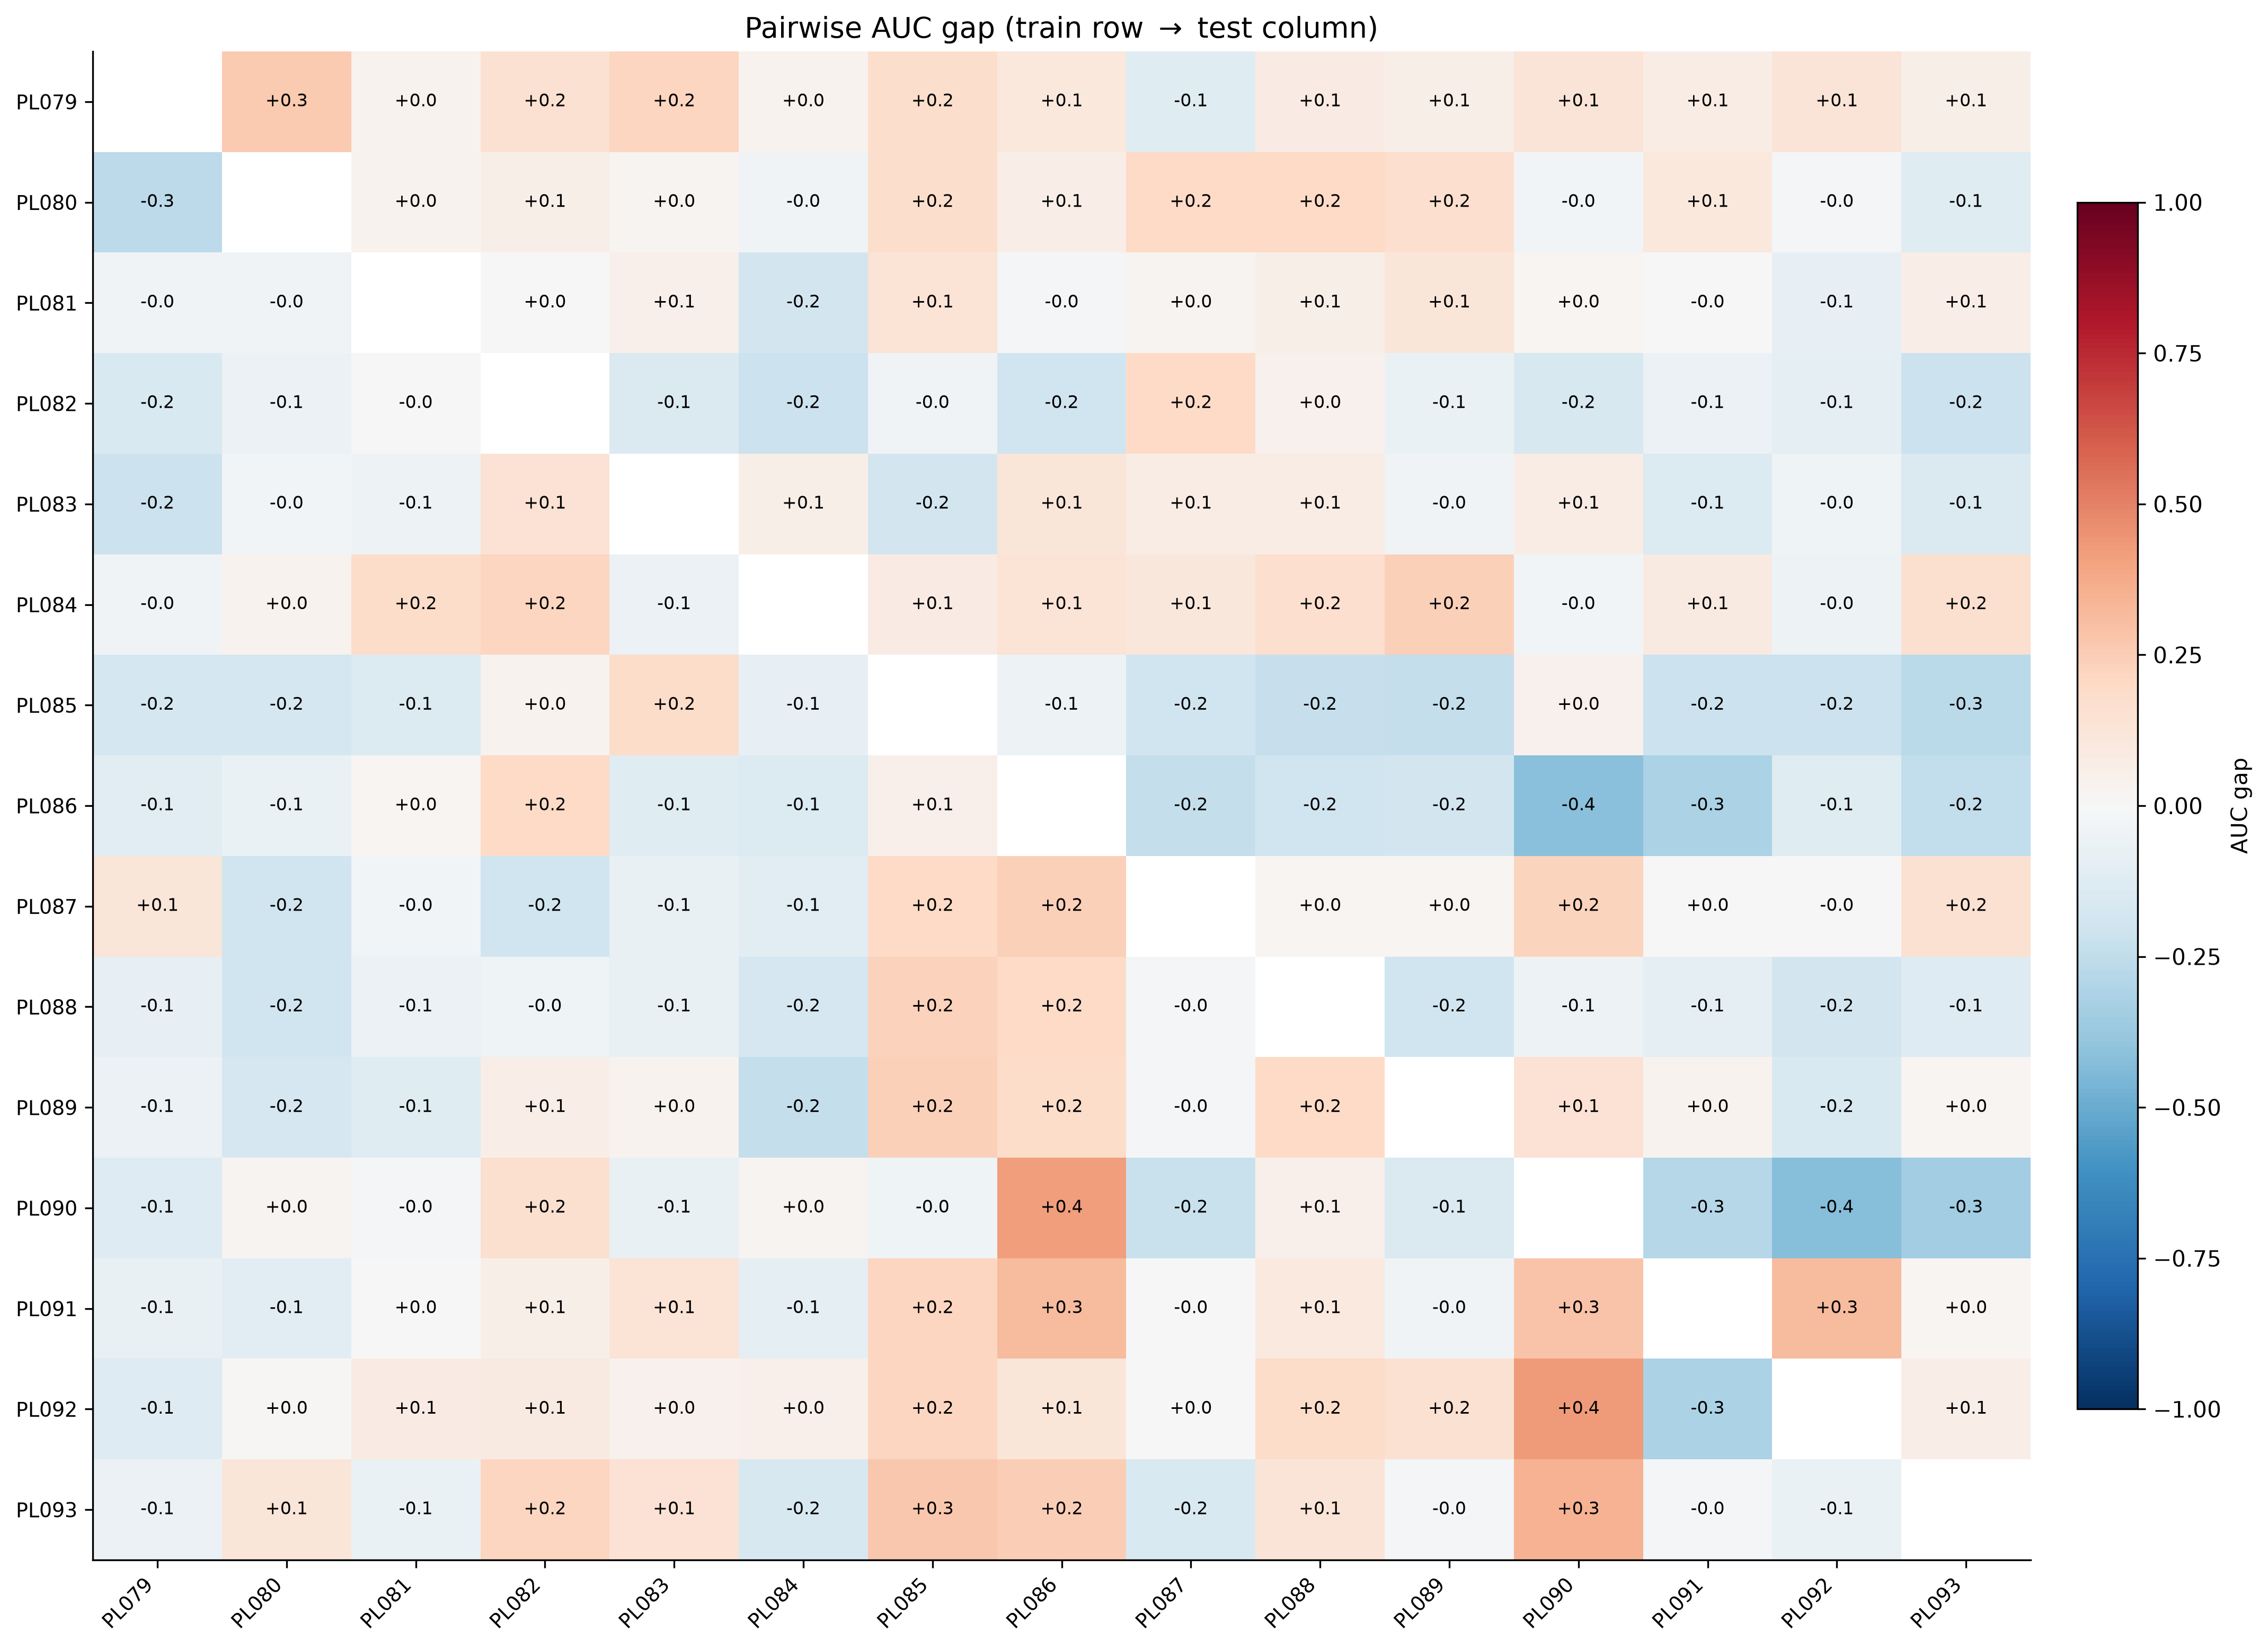
\includegraphics[width=0.9\textwidth]{results/multicohort/figures/F5_auc_gap_heatmap.png}
\caption{Pairwise AUC gap (train row, test column). Positive values (red) indicate worse external than internal performance; negative (blue) indicate better. The matrix is antisymmetric by construction. PL079 and PL084 are consistently poor senders; PL085 and PL086 are consistently poor receivers. Geodesic distance is symmetric and cannot capture this directional structure.}
\label{fig:aucgap}
\end{figure}


\section{Discussion}
\label{sec:discussion}

\paragraph{What the geometry detects.} Grassmannian geodesic distance reliably detects batch-induced subspace divergence in metabolomics data. The $z = 31.56$ separation from the permutation null is unambiguous: plates occupy distinct regions of the Grassmannian, and this structure is not an artifact of sample-level variance.

\paragraph{What the geometry does not predict.} Detecting batch structure is a necessary but not sufficient condition for predicting transportability failure. The prediction test ($\rho = 0.052$, $p = 0.598$) fails because the per-plate samples are too small for stable AUC estimation, not because the geometric measure lacks biological content. The geodesic distances and AUC gaps operate at different signal-to-noise ratios: geometry aggregates across all 1{,}022 features and is estimated from the full plate covariance, while AUC depends on $\sim$12 positive labels per plate.

\paragraph{Asymmetry.} The AUC gap is inherently asymmetric (training on plate $A$ and testing on $B$ differs from the reverse), while geodesic distance is symmetric. A directional geometric measure---such as the projection of the between-cohort shift onto the classification-relevant subspace---could capture this asymmetry. The Fisher-Rao confound score, which decomposes cross-cohort shift into batch and biological components, is a candidate for future work.

\paragraph{Limitations.}

\begin{itemize}
\item All results are retrospective on one public dataset (MTBLS7260). Generalization to other omics platforms, diseases, and sample sizes is untested.
\item Per-plate sample sizes ($\sim$72, $\sim$12 positives) are too small for the prediction test. A dataset with fewer, larger cohorts would be more informative.
\item Geodesic distances are compressed (CV 3.5\%), limiting the dynamic range for correlation. Datasets with cohorts from different instruments or laboratories would provide wider separation.
\item We use PCA subspaces as the representation. Nonlinear embeddings (autoencoders, foundation model representations) might produce different subspace structure.
\item The classifier (logistic regression) is a diagnostic tool, not an optimized clinical model. Stronger classifiers might produce different AUC gaps.
\end{itemize}

\paragraph{Conclusion.} Grassmannian geodesic distance provides a well-defined geometric test for batch structure in metabolomics: plates are detectably distinct ($z = 31.56$) and the closest and farthest plate pairs are identifiable from their principal angle spectra. Translating this geometric detection into quantitative prediction of classifier degradation remains open, and requires cohorts large enough that AUC estimates are precise enough for the geometric signal to resolve.

\bibliography{references}
\bibliographystyle{tmlr}

\end{document}
